
\documentclass{beamer}
\usetheme{ucl}

\usepackage[utf8]{inputenc}


%%% Increase the height of the banner: the argument is a scale factor >=1.0
%\setbeamertemplate{banner}[ucl][10.0]

%%% Change the colour of the main banner
%%% The background should be one of the UCL colours (except pink or white):
%%%   black,darkpurple,darkred,darkblue,darkgreen,darkbrown,richred,midred,
%%%   navyblue,midgreen,darkgrey,orange,brightblue,brightgreen,lightgrey,
%%%   lightpurple,yellow,lightblue,lightgreen,stone
\setbeamercolor{banner}{bg=darkpurple}
%\setbeamercolor{banner}{bg=yellow,fg=black}

%%% Add a stripe behind the banner
%\setbeamercolor{banner stripe}{bg=darkpurple,fg=black}

%%% The main structural elements
\setbeamercolor{structure}{fg=black}

%%% Author/Title/Date and slide number in the footline
\setbeamertemplate{footline}[author title date]

%%% Puts the section/subsection in the headline
% \setbeamertemplate{headline}[section]

%%% Puts a navigation bar on top of the banner
%%% For this to work correctly, the each \section command needs to be
%%% followed by a \subsection. Requires one extra compile.
% \setbeamertemplate{headline}[miniframes]
%%% Accepts an optional argument determining the width
% \setbeamertemplate{headline}[miniframes][0.3\paperwidth]


%%% Puts the frame title in the banner
%%% Won't work correctly with the above headline templates
%\useoutertheme{ucltitlebanner}
%%% Similar to above, but smaller (and puts subtitle on same line as title)
\useoutertheme[small]{ucltitlebanner}

%%% Gives block elements (theorems, examples) a border
% \useinnertheme{blockborder}
%%% Sets the body of block elements to be clear
% \setbeamercolor{block body}{bg=white,fg=black}

%%% Include CSML logo on title slide
%\titlegraphic{\includegraphics[width=0.16\paperwidth]{csml_logo}}

%%% Include CSML logo in bottom right corner of all slides
%\logo{\includegraphics[width=0.12\paperwidth]{csml_logo}}

%%% Set a background colour
% \setbeamercolor{background canvas}{bg=lightgrey}

%%% Set a background image
%%% Some sample images are available from the UCL image store:
%%%   https://www.imagestore.ucl.ac.uk/home/start
% \setbeamertemplate{background canvas}{%
%   \includegraphics[width=\paperwidth]{imagename}}



%%%%%% Some other settings that can make things look nicer
%%% Set a smaller indent for description environment
\setbeamersize{description width=2em}
%%% Remove nav symbols (and shift any logo down to corner)
\setbeamertemplate{navigation symbols}{\vspace{-2ex}}








\DeclareMathOperator{\Cov}{Cov}
\DeclareMathOperator{\Var}{Var}
\DeclareMathOperator{\E}{\mathbb{E}}
\DeclareMathOperator{\Proba}{\mathbb{P}}

\newcommand{\Covb}[2]{\ensuremath{\Cov\!\left[#1,#2\right]}}
\newcommand{\Eb}[1]{\ensuremath{\E\!\left[#1\right]}}
\newcommand{\Pb}[1]{\ensuremath{\Proba\!\left[#1\right]}}
\newcommand{\Varb}[1]{\ensuremath{\Var\!\left[#1\right]}}

% norm
\newcommand{\norm}[1]{\| #1 \|}

\newcommand{\indep}{\rotatebox[origin=c]{90}{$\models$}}





\usepackage{mathptmx,amsmath,amssymb,graphicx,bibentry,bbm,ragged2e}
\usepackage[english]{babel}

\makeatletter

\newcommand{\noun}[1]{\textsc{#1}}
\newcommand{\jitem}[1]{\item \begin{justify} #1 \end{justify} \vfill{}}
\newcommand{\sframe}[2]{\frame{\frametitle{#1} #2}}

\newenvironment{centercolumns}{\begin{columns}[c]}{\end{columns}}
%\newenvironment{jitem}{\begin{justify}\begin{itemize}}{\end{itemize}\end{justify}}



%\usetheme{Warsaw}
%\setbeamertemplate{footline}[text line]{}
%\setbeamertemplate{headline}{}
%\setbeamercolor{structure}{fg=purple!50!blue, bg=purple!50!blue}

%\setbeamersize{text margin left=15pt,text margin right=15pt}

%\setbeamercovered{transparent}


\@ifundefined{showcaptionsetup}{}{%
 \PassOptionsToPackage{caption=false}{subfig}}
\usepackage{subfig}

\usepackage[utf8]{inputenc}
\usepackage[T1]{fontenc}

\usepackage{multirow}


\makeatother

\def \draft {1}

\usepackage{xparse}
\usepackage{ifthen}
\DeclareDocumentCommand{\comment}{m o o o o}
{\ifthenelse{\draft=1}{
    \textcolor{red}{\textbf{C : }#1}
    \IfValueT{#2}{\textcolor{blue}{\textbf{A1 : }#2}}
    \IfValueT{#3}{\textcolor{ForestGreen}{\textbf{A2 : }#3}}
    \IfValueT{#4}{\textcolor{red!50!blue}{\textbf{A3 : }#4}}
    \IfValueT{#5}{\textcolor{Aquamarine}{\textbf{A4 : }#5}}
 }{}
}
\newcommand{\todo}[1]{
\ifthenelse{\draft=1}{\textcolor{red!50!blue}{\textbf{TODO : \textit{#1}}}}{}
}




\begin{document}

\title[Models of urban morphogenesis]{Models of urban morphogenesis to link urban form and function}
\author[J. Raimbault]{J.~Raimbault$^{1,2,3\ast}$\\\medskip
$^{\ast}$\texttt{j.raimbault@ucl.ac.uk}
}

\institute[UCL]{$^{1}$CASA, UCL\\
$^{2}$UPS CNRS 3611 Complex Systems Institute Paris\\
$^{3}$UMR CNRS 8504 G{\'e}ographie-cit{\'e}s
}




\date[15th November 2019]{TQG Debates 2019\\
3.1: Fractals and Multi-fractals\\
November 15th 2019
}

\frame{\maketitle}


% The understanding of processes driving urban growth is a necessary step before designing and implementing policies for territorial sustainability. At the intermediate scale of metropolitan areas, urban form, in the sense of the spatial distribution of settlements and activities, has a complex relation with urban function. We propose in this presentation to investigate models of urban growth at such a scale, in the conceptual framework of morphogenesis that we define as the emergence of form and function and their strong coupling. We first investigate a simple reaction-diffusion model of urban morphogenesis for population density, capturing the contradictory processes of urban concentration and dispersal. The model is calibrated on real density data for Europe and shown to reproduce most of existing territorial forms. It is also tested on some large areas across the world using the Global Human Settlement Layer database. We then introduce urban functions in an indirect way  by coupling this model with road network generation models, since networks shape accessibility landscapes to amenities. Multiple network generation heuristics are compared and shown to be complementary to reproduce existing coupled patterns of urban form and network topology. We finally discuss potential links with urban fractal properties and developments towards more realistic data-driven morphogenesis models which could be applied to the design and test of policies to increase sustainability. 



\section{Introduction}


\sframe{Complex processes of Urban Morphogenesis}{

\centering

% center of Paris
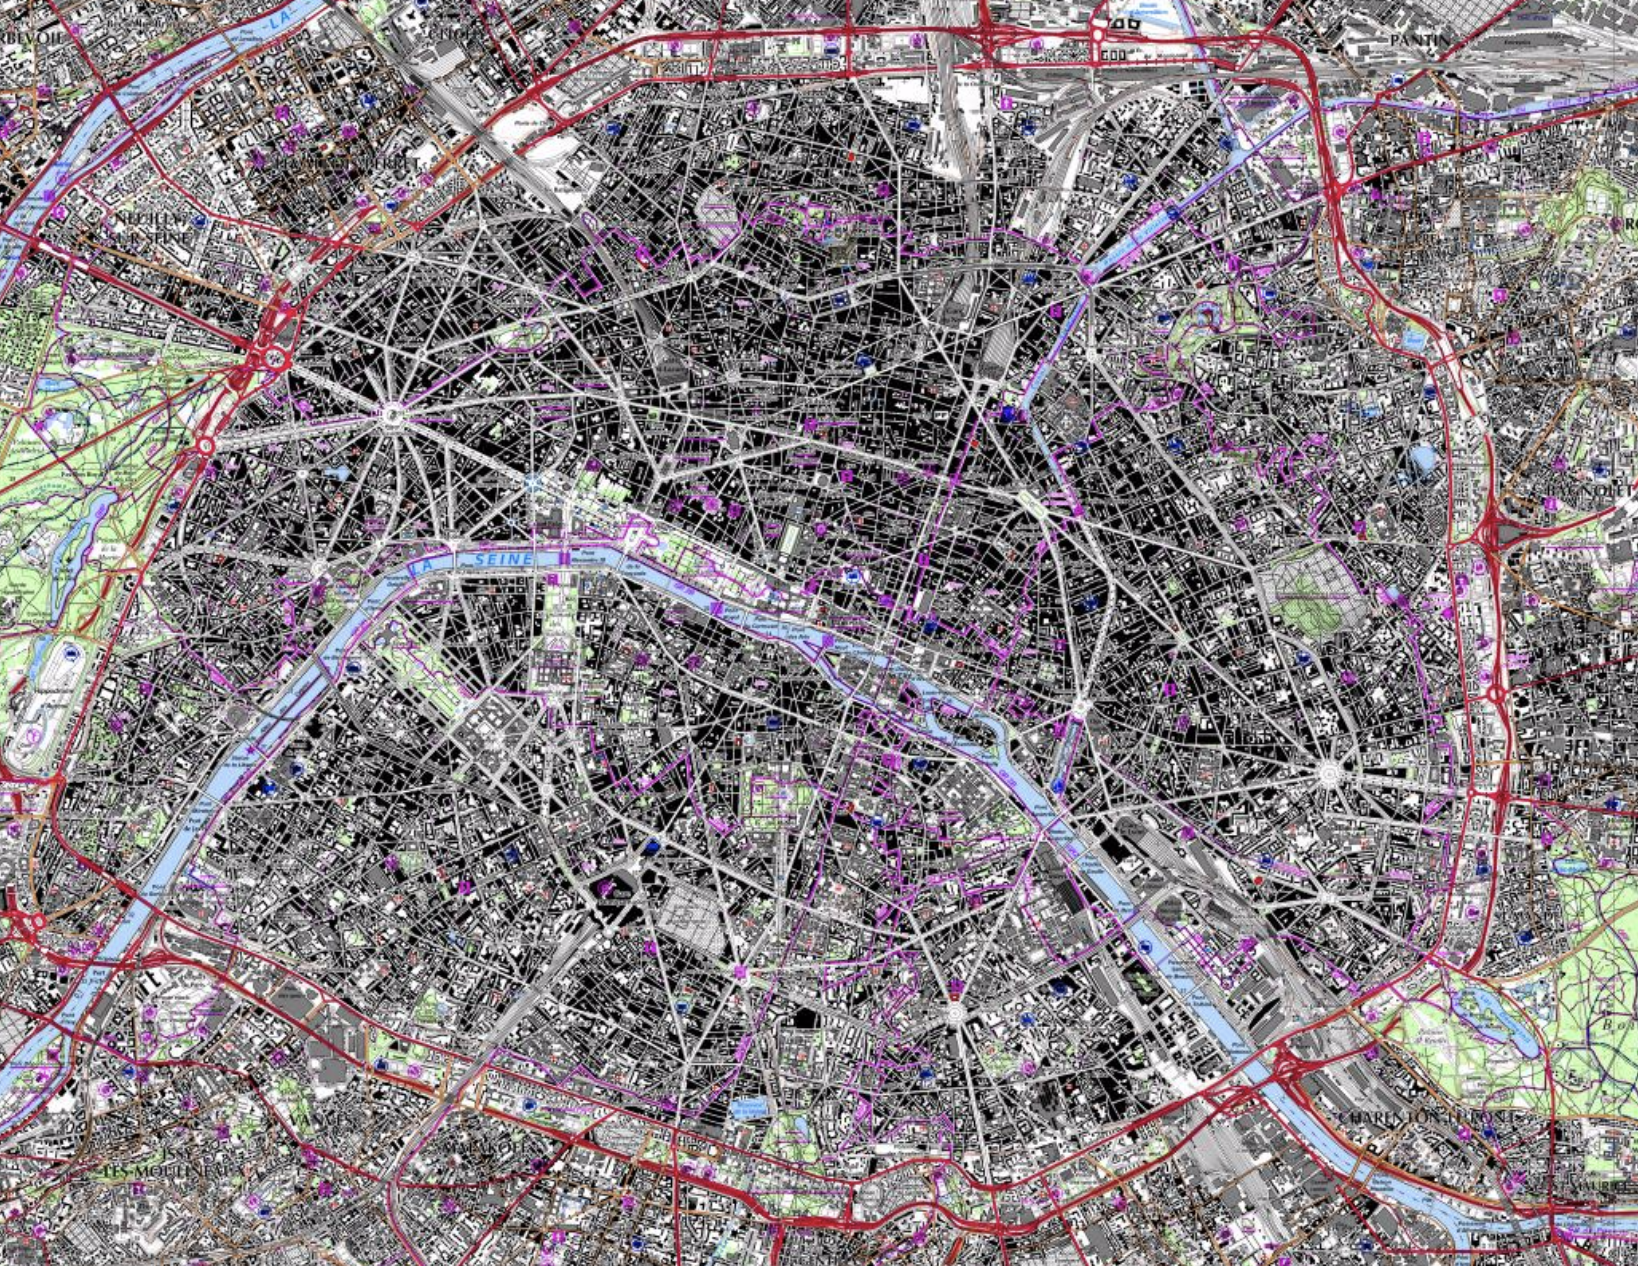
\includegraphics[width=0.88\textwidth]{figures/intro_paname}

\footnotesize\textit{Source: Geoportail}
}

\sframe{Complex processes of Urban Morphogenesis}{

\centering

% large bp
\includegraphics[width=0.9\textwidth]{figures/intro_bp}

\footnotesize\textit{Source: Geoportail}
}



\sframe{What is Morphogenesis ?}{

\textbf{Morphogenesis} (\textit{Oxford dictionary}) 
\begin{enumerate}
\item \textit{Biology} : The origin and development of morphological characteristics
\item \textit{Geology} : The formation of landforms or other structures.
\end{enumerate}

\bigskip

\textbf{History of the notion}

$\rightarrow$ Started significantly with embryology around 1930~\cite{abercrombie1977concepts} 

$\rightarrow$ Turing's 1952 paper~\cite{turing1952chemical}, linked to the development of Cybernetics

$\rightarrow$ first use in 1871, large peak in usage between 1907-1909, increase until 1990, decrease until today. \textit{Scientific fashion ?}


}





\sframe{What is Morphogenesis ? Examples}{

% illustrations : ants, geomorphology, neurons, self-assembly ; ARBOTRON ; paper nature aile avion
% all from netlogo library ? would be nice illustration of generative nature


% remark : do not put classical biological example to show how it has percolated to other fields

\vspace{-0.3cm}

\includegraphics[width=\textwidth,height=0.82\textheight]{figures/intro_examples}

\justify

\vspace{-0.5cm}

\footnotesize\textit{Sources (in order by column). Ants, Erosion, Game of Life: NetLogo Library; Arbotron \cite{jun2005formation}; Industrial design \cite{Aage:2017aa}; Swarm chemistry \cite{sayama2007decentralized}}
% sources : ants netlogo ; erosion netlogo ; arbotron 
%  inge : 

}



\sframe{Defining Morphogenesis}{

% precise notions and defs

\justify

\textit{Proposition of an interdisciplinary definition}

\bigskip




\textbf{Meta-epistemological framework of imbricated notions:}

Self-organization $\supsetneq$ Morphogenesis $\supsetneq$ Autopoiesis $\supsetneq$ Life


\bigskip

\textbf{Properties:}

\begin{itemize}
\item Architecture links form and function
\item Emergence strength~\cite{bedau2002downward} increases with notion depth, as bifurcations~\cite{thom1974stabilite}
\end{itemize}

\bigskip

\textbf{Definition of Morphogenesis :} \textit{Emergence of the form and the function in a strongly coupled manner, producing an emergent architecture \cite{doursat2012morphogenetic}}



}



\sframe{Which models for Urban Morphogenesis ?}{

% why modeling, exemple of rbd
% -> champ ; difficultés ("verrous". rq : j'aime pas la metaphore du verrou, trop cadrant et suppose que deja construit et qu'il suffit d'ouvrir. demarche epistemo de co-evol des connaissances, ni inductif ni deductif. il faut contruire. horizons d'exploration plus appropriés. rejoint l'idee de faire rentrer dans "cadre analytique" : cases prédéfinies, alors qu'il s'agit au contraire de définir ces cases. -> relire hdr arnaud

\justify

\begin{columns}
\column{0.35\textwidth}
\centering
\includegraphics[width=\textwidth]{figures/intro_RBD_lattice}\\
\footnotesize\textit{Example: a basic hybrid model based on elementary processes for density and network \cite{raimbault2014hybrid}}
\column{0.6\textwidth}
\justify

%\vspace{-1cm}

$\rightarrow$\textit{At the crossroad between Urban Simulation and Artificial Life, few models try to integrate and explain the link between Urban Form and Function}

\medskip

$\rightarrow$\textit{Importance of parcimonious, stylized models: modeling as a tool to understand processes}

\end{columns}

\bigskip

\textbf{Research Objective : } Explore simple models to capture morphogenesis based on abstract representation of urban processes; test their ability to reproduce existing urban systems.



}


\section{Reaction-diffusion model}


\sframe{A simple Reaction-diffusion model}{

% comment Arnaud : reaction-diffusion ?

% model rationale and processes


\justify

$\rightarrow$ Crucial role of the interplay between concentration forces and dispersion forces~\cite{fujita1996economics} in keeping Urban Systems at the border of chaos

\bigskip

$\rightarrow$ Potentiality of aggregation mechanisms (such as Simon model) to produce power laws \cite{dodds2017simon}

\bigskip

$\rightarrow$ Link with Reaction-diffusion approaches in Morphogenesis~\cite{turing1952chemical}

\bigskip

$\rightarrow$ Extension of a DLA-type model introduced by \cite{batty1991generating}, with simple abstract processes of population aggregation and diffusion

\bigskip
\bigskip

{\tiny

Raimbault, J. (2018). Calibration of a density-based model of urban morphogenesis. PloS one, 13(9), e0203516.
}

}

\sframe{Model Formalization}{

% model formalization and indicators

$\rightarrow$ Grid world with cell populations $\left(P_i\left(t\right)\right)_{1\leq i\leq N^2}$.

\bigskip

$\rightarrow$ At each time step:


\begin{enumerate}
\item Population growth with exogenous rate $N_G$, attributed independently to a cell following a preferential attachment of strength $\alpha$
%\begin{equation}
%\Pb{P_i(t+1)=P_i(t)+1|P(t+1)=P(t)+1}=\frac{(P_i(t)/P(t))^{\alpha}}{\sum(P_i(t)/P(t))^{\alpha}}
%\end{equation}
%The attribution being uniformly drawn if all population are equal to 0.
\item Population is diffused $n_d$ times with strength $\beta$
\end{enumerate}

\bigskip

$\rightarrow$ Stopping criterion: fixed maximal population $P_m$.

%To avoid bord effects such as reflecting diffusion waves, border cells diffuse their due proportion outside of the world, implying that the total population at time $t$ is strictly smaller than $N_G\cdot t$.

\bigskip

$\rightarrow$ Output measured by morphological indicators: Moran index, average distance, rank-size hierarchy, entropy.


}


\sframe{Generating Population Distributions}{


% examples : fig 2 of paper

\centering

\includegraphics[height=0.8\textheight]{figures/density_Fig2}

\footnotesize\textit{Examples of generated territorial shapes}

}


\sframe{Model behavior}{

\centering

\includegraphics[width=0.9\textwidth]{figures/density_Fig3}

\footnotesize\textit{Phase transitions of indicators unveiled by exploration of the parameter space (80000 parameter points, 10 repetitions each)}


}




\sframe{Path-dependence and frozen accidents}{

\centering

\includegraphics[width=0.8\textwidth]{figures/density_Fig4}

\footnotesize\textit{Illustration of path-dependence in a simplified one-dimensional version of the model: cell trajectories in time for 9 independent repetitions from the same initial configuration.}


}


\sframe{Empirical Data for Calibration}{

% comments Arnaud : Quel lien avec les slides avant et après ? "Real" : le terme me paraît discutable : données empiriques plutôt ?
%  Décrire les données car ici tu passes directement aux indicateurs

\begin{columns}
\column{0.6\textwidth}
\centering
\includegraphics[width=\textwidth]{figures/density_indics_morpho_discrquantiles}
\column{0.3\textwidth}
\centering
\includegraphics[width=\textwidth]{figures/density_cluster_pca_k5_morpho}\\
\includegraphics[width=\textwidth]{figures/density_cluster_map_k5_morpho}
\end{columns}

\justify

\footnotesize\textit{Computation of morphological indicators on population density data for Europe (shown here on France), morphological classification.}

}



\sframe{Model Calibration}{

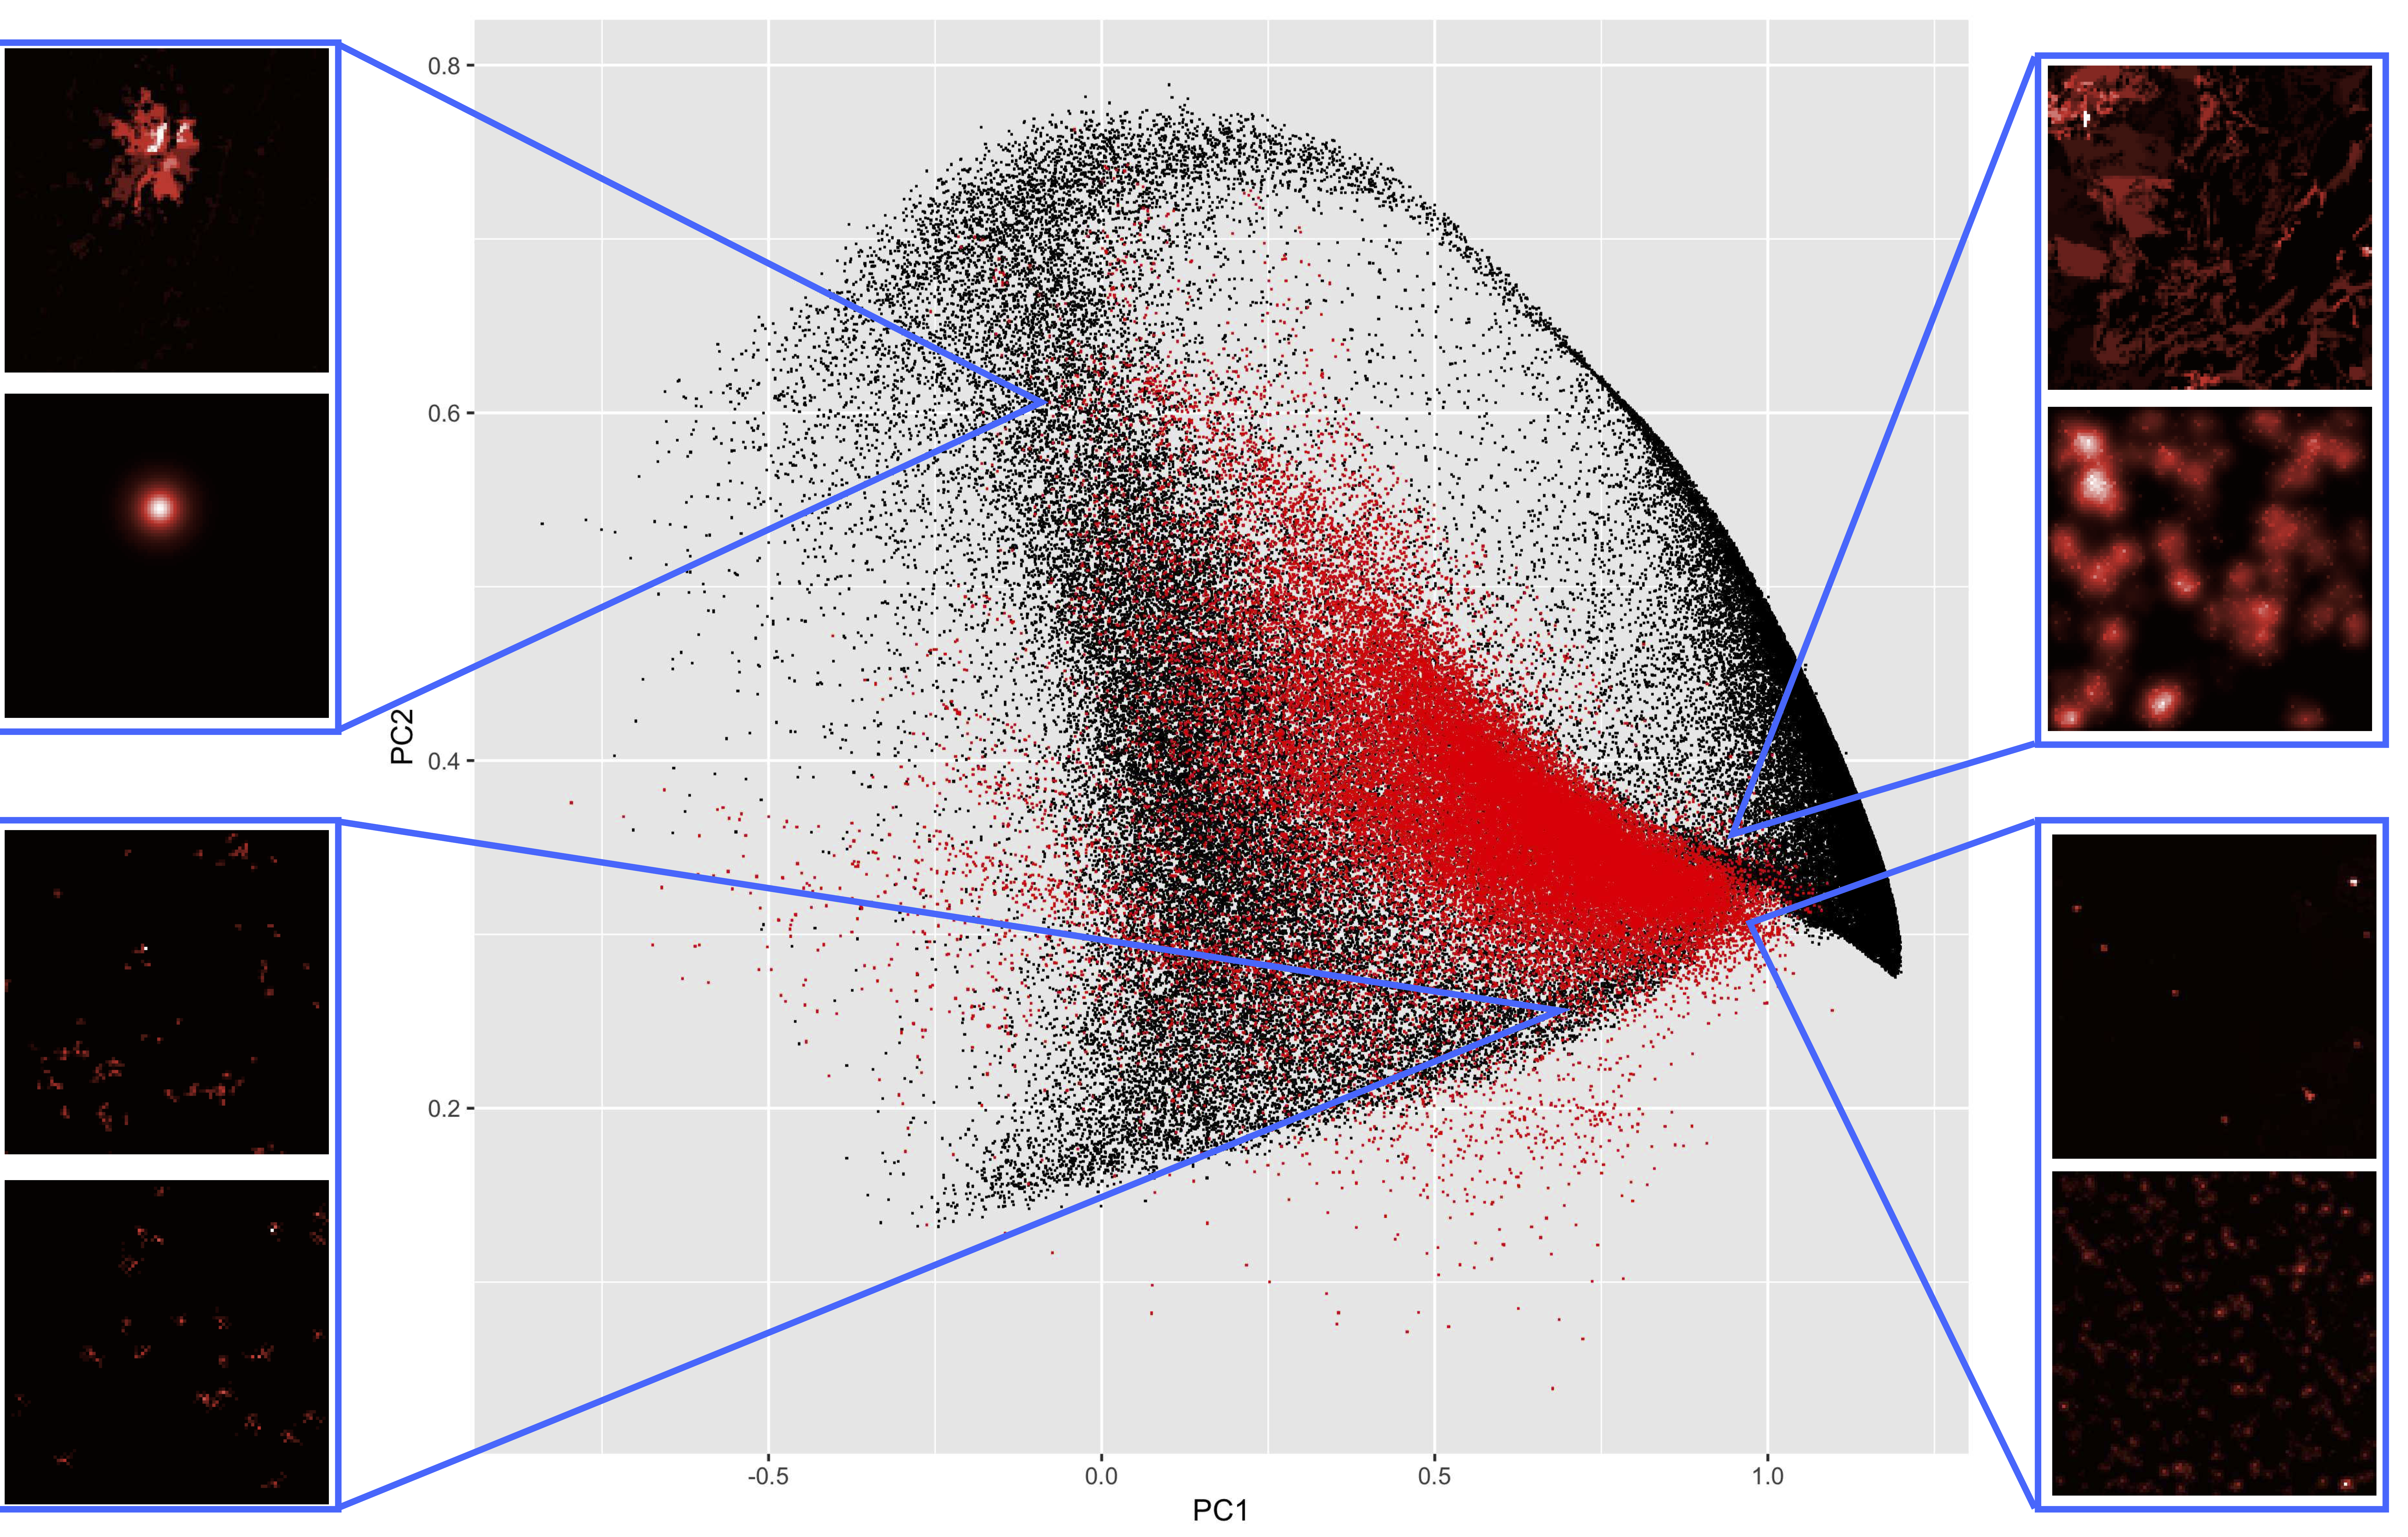
\includegraphics[width=0.9\textwidth]{figures/density_synth}

\footnotesize\textit{Brute force calibration by exploring the parameter space. Reproduction of most existing configuration in the morphological sense (here in principal plan).}

}



\sframe{Model Targeted Exploration}{

\centering

\includegraphics[width=0.8\textwidth]{figures/density_Fig6}

\footnotesize\textit{Potentialities of targeted model explorations: here feasible space using Pattern Space Exploration algorithm \cite{10.1371/journal.pone.0138212}.}

}



\section{Co-evolution model}


\sframe{Including more complex processes ?}{

% transition : representation of territories

\textit{Which ontology to include more complex functional properties ?}

\medskip

$\rightarrow$ Territorial systems as the strong coupling between territories and (potential and realized) networks \cite{dupuy1987vers}.

\medskip

$\rightarrow$ Networks convey functional notions of centralities and accessibility, among others; have furthermore proper topological properties.


}



\sframe{Interactions between networks and territories}{

\justify

\begin{center}
\includegraphics[width=0.45\linewidth]{figures/accessp_withbridge_prd_EN.png}
\hspace{0.1cm}
\includegraphics[width=0.52\linewidth]{figures/avgaccess_facet.png}

\end{center}

\medskip

%\vspace{-0.5cm}

%\begin{justify}
\textit{Accessibility as part of complex processes of co-evolution between transportation networks and territories.}

%\end{justify}

\nocite{raimbault2018evolving}

\medskip

\tiny

Raimbault, J. (2019). Evolving accessibility landscapes: mutations of transportation networks in China. In Aveline-Dubach, N., ed. \textit{Pathways of sustainable urban development across China - the cases of Hangzhou, Datong and Zhuhai}, pp 89-108. Imago. ISBN:978-88-94384-71-0

}



\sframe{A Morphogenesis Model of co-evolution}{

\justify

\vspace{-1cm}

$\rightarrow$ Coupled grid population distribution and vector transportation network, following the core of \cite{raimbault2014hybrid}

\medskip

$\rightarrow$ Local morphological and functional variables determine a patch-value, driving new population attribution through preferential attachment ; combined to population diffusion (reaction-diffusion processes studied before)


\medskip

$\rightarrow$ Network growth is also driven by morphological, functional and local network measures, following diverse heuristics corresponding to different processes (multi-modeling)

\medskip

\textit{Local variables and network properties induce feedback on both, thus a strong coupling capturing the \textbf{co-evolution}}

\bigskip

{
\tiny

Raimbault, J. (2019). An urban morphogenesis model capturing interactions between networks and territories. In The Mathematics of Urban Morphology (pp. 383-409). Birkhäuser, Cham.

\medskip

Raimbault, J. (2018). Multi-modeling the morphogenesis of transportation networks. In Artificial Life Conference Proceedings (pp. 382-383).

}


}



\sframe{Model : Specification}{

\includegraphics[width=\textwidth]{figures/coevol_mesocoevol}

}



\sframe{Network Generation}{

At fixed time steps :

\begin{enumerate}
	\item Add new nodes preferentially to new population and connect them
	\item \justify Variable heuristic for new links, among: nothing, random, gravity-based deterministic breakdown, gravity-based random breakdown (from \cite{schmitt2014modelisation}), cost-benefits (from \cite{louf2013emergence}), biological network generation (based on \cite{tero2010rules})
\end{enumerate}

\medskip

\centering

\frame{\includegraphics[height=0.31\textwidth]{figures/coevol_example-bio-process-1}}\hspace{0.2cm}
\frame{\includegraphics[height=0.31\textwidth]{figures/coevol_example-bio-process-1-tick80}}

\footnotesize

\textit{Intermediate stage for biological network generation}

}




\sframe{Generated Urban Shapes: Urban Form}{

\centering

\frame{\includegraphics[width=0.28\textwidth]{figures/coevol_example_synthsetup}}\hspace{0.1cm}
\frame{\includegraphics[width=0.28\textwidth]{figures/coevol_example_form-accessonly}}\hspace{0.1cm}
\frame{\includegraphics[width=0.28\textwidth]{figures/coevol_example_form-droadonly}}\\\vspace{0.1cm}
\frame{\includegraphics[width=0.28\textwidth]{figures/coevol_example_form-bwonly}}\hspace{0.1cm}
\frame{\includegraphics[width=0.28\textwidth]{figures/coevol_example_form-closenessonly}}\hspace{0.1cm}
\frame{\includegraphics[width=0.28\textwidth]{figures/coevol_example_form-poponly}}

\footnotesize\textit{In order: setup; accessibility driven; road distance driven; betweenness driven; closeness driven; population driven.}

}






\sframe{Generated Urban Shapes: Network}{


\centering

\frame{\includegraphics[width=0.28\textwidth]{figures/coevol_example_nw-connection}}\hspace{0.1cm}
\frame{\includegraphics[width=0.28\textwidth]{figures/coevol_example_nw-random}}\hspace{0.1cm}
\frame{\includegraphics[width=0.28\textwidth]{figures/coevol_example_nw-gravity}}\\\vspace{0.1cm}
\frame{\includegraphics[width=0.28\textwidth]{figures/coevol_example_nw-rndbrkdwn}}\hspace{0.1cm}
\frame{\includegraphics[width=0.28\textwidth]{figures/coevol_example_nw-cost}}\hspace{0.1cm}
\frame{\includegraphics[width=0.28\textwidth]{figures/coevol_example_nw-bio}}

\footnotesize\textit{In order: connection; random; deterministic breakdown; random breakdown; cost-driven; biological.}

}



\sframe{Results : Network Heuristics}{

\justify

\textit{Comparison of feasible space for network indicators with fixed density}

\bigskip

\includegraphics[width=0.52\textwidth,height=0.6\textheight]{figures/coevol_feasible_space_withreal_pca_bymorph}
\includegraphics[width=0.43\textwidth,height=0.6\textheight]{figures/coevol_distance_real_bymorph}

\footnotesize

\textit{(Left) Feasible spaces by morphological class and network heuristic; (Right) Distribution of distances to topologies of real networks}

}


\sframe{Results : Calibration}{

\justify

\vspace{-0.5cm}

Calibration (model explored with OpenMole~\cite{reuillon2013openmole}, $\sim 10^6$ model runs) at the first order on morphological and topological objectives, and on correlations matrices.

\bigskip

\begin{columns}
\column{0.4\textwidth}
\centering
\includegraphics[width=\textwidth]{figures/coevol_pca_allobjs}
\column{0.2\textwidth}
\includegraphics[width=\textwidth]{figures/coevol_pca_morpho_byheuristic}\\
\includegraphics[width=\textwidth]{figures/coevol_pca_network_byheuristic}
\column{0.4\textwidth}
\includegraphics[width=\textwidth]{figures/coevol_corrs-distrib_rhoasize4}

\end{columns}

\footnotesize\textit{(Left) Full indicator space; (Middle) Morphological and Topology, by network heuristic; (Right) Distance distribution for cumulated distance for indicators and correlations.}

}


\sframe{Results : Causality Regimes}{

\textit{Unsupervised learning on lagged correlations between local variables unveils a diversity of causality regimes}

$\rightarrow$ Link between \emph{co-evolution regime} and morphogenetic properties of the urban system

% comment Arnaud : le genre d’affirmation qu’il faut réussir à exprimer également du point de vue de l’objet étudié : qu’est-ce que ça veut dire pour la morphogénèse urbaine ?

\medskip

\centering

\includegraphics[width=0.52\textwidth,height=0.55\textheight]{figures/coevol_centertrajs}
\includegraphics[width=0.4\textwidth,height=0.55\textheight]{figures/coevol_cluster-params}

\footnotesize\textit{(Left) Lagged correlation profiles of cluster centers; (Right) Distribution of regimes across parameter space}

}


\section{Discussion}



\sframe{Discussion}{

\justify

\vspace{-1cm}

\textbf{Implications}

$\rightarrow$ This rather simple model reproduces most of existing urban forms in Europe for both population distribution and road network : which intrinsic dimension to the urban system and its morphological aspect ?

$\rightarrow$ Ability to reproduce static correlations and a variety of dynamical lagged correlation regimes suggests that the model captures some of the processes of co-evolution

% implications for morphogenesis ?

\bigskip

\textbf{Developments}


$\rightarrow$ Towards a dynamical calibration ? Need of dynamical data

$\rightarrow$ Investigate the link between spatial non-stationarity and non-ergodicity through simulation by the model

$\rightarrow$ Compare network generation in a ``fair'' way (correcting for additional parameters, open question for models of simulation)


}


\sframe{Link with fractals}{


\justify

% \cite{nelson1988modeling} lung morphogenesis
% \cite{matsuyama1993fractal} DLA model for bacteria colony morphogenesis

% original urban DLA approach Batty

% Open Q / future work ?
%  - link between fractal measures of urban form and other measures
%  - multiscale - multifractal model ? 

Morphogenesis and fractals already linked in the biological literature: for example \cite{nelson1988modeling} with network morphogenesis, \\\cite{matsuyama1993fractal} with a DLA model for bacteria self-organization

\bigskip

Also links in Urban Science: DLA model \cite{batty1991generating}, fractal models of urban growth \cite{frankhauser2008fractal}


\bigskip
\bigskip

\textbf{Open questions:}

\medskip

$\rightarrow$ Formal link between fractal properties and the dynamics of form and function \cite{batty1999research}

\medskip

$\rightarrow$ Relating fractal indicators of urban form with other dimensions

\medskip

$\rightarrow$ Link between multi-fractal properties \cite{salat2017multifractal} and multi-scalar models of urban systems \cite{raimbault:halshs-02351722}


}


\sframe{Towards policy applications}{

% more data

\justify

\textbf{More realistic models?}

\medskip

$\rightarrow$ Introducing more concrete ontologies, economic processes \\
\cite{bonin2014modelisation}, qualitative differentiation \cite{bonin2012modele}, governance processes \cite{le2015modeling}

\medskip

$\rightarrow$ Possible bridges with Land-use change models/Land-use Transport models \cite{wegener2004land}, with systems of cities models\\
 \cite{pumain2017urban}

\medskip

\textbf{More data-driven models?}

\medskip

$\rightarrow$ Work in progress: calibration of the reaction-diffusion model on world urban areas with the Global Human Settlements Layer database

\medskip

$\rightarrow$ Link with sustainability indicators: GHG emissions, economics, etc. \cite{raimbault2019multi}

\medskip

$\rightarrow$ Study models on hybrid synthetic data \cite{raimbault2018space}: systematic conclusions for policies



}




\sframe{Conclusion}{


\justify

$\rightarrow$ A novel model of urban morphogenesis at the mesoscopic scale systematically explored: \textbf{need for more coupling and comparison of models.}

\medskip

$\rightarrow$ At the macro scale of the system of cities? \textbf{Need for multi-scale models.}

\medskip

$\rightarrow$ With more refined urban characteristics and other dimensions ? \textbf{Need for more interdisciplinarity.}

\bigskip
\bigskip
\bigskip

\footnotesize{ - Code, data and results available at\\ \texttt{https://github.com/JusteRaimbault/CityNetwork}\\
- Acknowledgments: Thanks to the \textit{European Grid Infrastructure} and its \textit{National Grid Initiatives} (\textit{France-Grilles} in particular) to give the technical support and the infrastructure.

}

}



\section*{Reserve slides}


\sframe{Reserve slides}{

\centering

\Large

\textbf{Reserve Slides}

}




%%%%%%%%%%%%%%%%%
%\section*{Morphogenesis}



\sframe{Morphogenesis Overview}{
% other numerous examples of fields/case of application

\cite{bourgine2010morphogenesis} : interdisciplinary workshop on morphogenesis

\bigskip

$\rightarrow$\textit{To what extent the notion is indeed transdisciplinary, i.e. are there common definitions across disciplines ? What are the concepts shared or the divergence ?}


\begin{itemize}
\item \textbf{Biology}
\begin{itemize}
\item External phenotype morphogenesis (ant colony)~\cite{minter2012morphogenesis} \item Symbiosis of species~\cite{chapman1998morphogenesis}
\item Botany~\cite{lord1981cleistogamy}
\end{itemize}
\item \textbf{Social Sciences} : Archeology~\cite{renfrew1978trajectory}
\item \textbf{Epistemology} : \cite{gilbert2003morphogenesis}
\item \textbf{Artificial Intelligence} : From self-assembly to Morphogenetic Engineering~\cite{doursat2013review}. Synthetic Biology ?
\item \textbf{Geomorphology} : dunes formation~\cite{douady2011dunes}
\item \textbf{Physics} : Arbotrons playing Tetris ?
\item etc\ldots
\end{itemize}




}



\sframe{Morphogenesis concepts}{

\begin{itemize}
\item \justify \textbf{Morphogenesis and Self-Organisation} : when does a system exhibit an architecture ? Insights from Morphogenetic Engineering
\cite{doursat2013review}. Architecture : the relation between the form and the function ?
\medskip
\end{itemize}
\begin{itemize}
\item \justify\textbf{Scales, Units and Boundaries} From local interactions to global information flow (Holland's \emph{signal and boundaries}~\cite{holland2012signals}: morphogenesis as the development of Complex Adaptive Systems ?)
\medskip
\end{itemize}
\begin{itemize}
\item \justify \textbf{Symmetry and Bifurcations} : on quantitative becoming qualitative. Ren{\'e} Thom's \emph{theory of catastrophes}~\cite{thom1974stabilite}
\medskip
\end{itemize}
\begin{itemize}
\item \justify \textbf{Life and Death} : link with autopoiesis and cognition\\
\cite{bourgine2004autopoiesis} ; co-evolution of subsystems as an alternative definition ? In psychology, attractors of the mind.
\end{itemize}


}


\sframe{Catastrophe Theory}{

% brief rapide sur theorie des catastrophes

A system is viewed as its internal state $X_w$, where $w\in W$ is a control parameter.

\bigskip

Catastrophe set $K \subset W$ is where the system endures phase transition.

\bigskip

Thom classified possible topologies for $K$ depending on the dimension of $W$.

}



\sframe{Modeling Urban Morphogenesis}{

\justify

\cite{makse1998modeling} correlated growth; 

\cite{10.1371/journal.pone.0133780} multi-scale migration and percolation; 

\cite{bonin2012modele} qualitative differentiation of urban function; 

\cite{achibet2014model} procedural model at the micro-scale 

}




%%%%%%%%%%%%%%%%%
%\section*{Density Morphogenesis}





\sframe{Model classification : PDE}{

% derived PDE

The one-dimensional model verifies the PDE :

\begin{equation}\label{eq:pde}
\begin{split}
\delta t \cdot \frac{\partial p}{\partial t} \textrm{ = } \frac{N_G \cdot p^{\alpha}}{P_{\alpha}(t)} \textrm{ + } \frac{\alpha \beta \left(\alpha - 1\right) \delta x^2}{2}\cdot \frac{N_G \cdot p^{\alpha-2}}{P_{\alpha}\left(t\right)} \cdot \left(\frac{\partial p}{\partial x}\right)^2\\
\textrm{ + } \frac{\beta \delta x^2}{2} \cdot \frac{\partial^2 p}{\partial x^2} \cdot\left[ 1 \textrm{ + } \alpha \frac{N_G p^{\alpha - 1}}{P_{\alpha(t)}} \right]
\end{split}
\end{equation}

}


\sframe{Stationary behavior of 1D model}{
\centering
\includegraphics[width=\textwidth]{figures/density_stationary}
}

\sframe{Stationary behavior of 1D model}{
\centering
\includegraphics[width=0.48\textwidth]{figures/density_pmax_alpha}
\includegraphics[width=0.48\textwidth]{figures/density_pmax_logbeta}

}



\sframe{Morphological indicators}{

\begin{enumerate}
\item Rank-size slope $\gamma$, given by $\ln \left( P_{\tilde{i}}/P_0\right) \sim k \textrm{ + } \gamma\cdot \ln \left(\tilde{i}/i_0\right)$ where $\tilde{i}$ are the indexes of the distribution sorted in decreasing order.
\item Entropy of the distribution:
\begin{equation}
\mathcal{E} \textrm{ = } \sum_{i=1}^{M}\frac{P_i}{P}\cdot \ln{\frac{P_i}{P}}
\end{equation}
$\mathcal{E}\textrm{ = }0$ means that all the population is in one cell whereas $\mathcal{E}\textrm{ = }0$ means that the population is uniformly distributed.
\item Spatial-autocorrelation given by Moran index, with simple spatial weights given by $w_{ij} \textrm{ = } 1/d_{ij}$
\[
I \textrm{ = } M \cdot \frac{\sum_{i\neq j} w_{ij} \left(P_i - \bar{P}\right)\cdot\left(P_j - \bar{P}\right)}{\sum_{i\neq j} w_{ij} \sum_{i}{\left( P_i - \bar{P}\right)}^2}
\]
\item Mean distance between individuals
\[
\bar{d} \textrm{ = } \frac{1}{d_M}\cdot \sum_{i<j} \frac{P_i P_j}{P^2} \cdot d_{ij}
\]
where $d_M$ is a normalisation constant
\end{enumerate}



}


\sframe{Model behavior : Convergence}{

Large number of repetitions show good convergence properties

% hist examples

\includegraphics[width=0.5\textwidth]{figures/density_hist_moran}
\includegraphics[width=0.5\textwidth]{figures/density_hist_slope}

}


\sframe{Model behavior}{


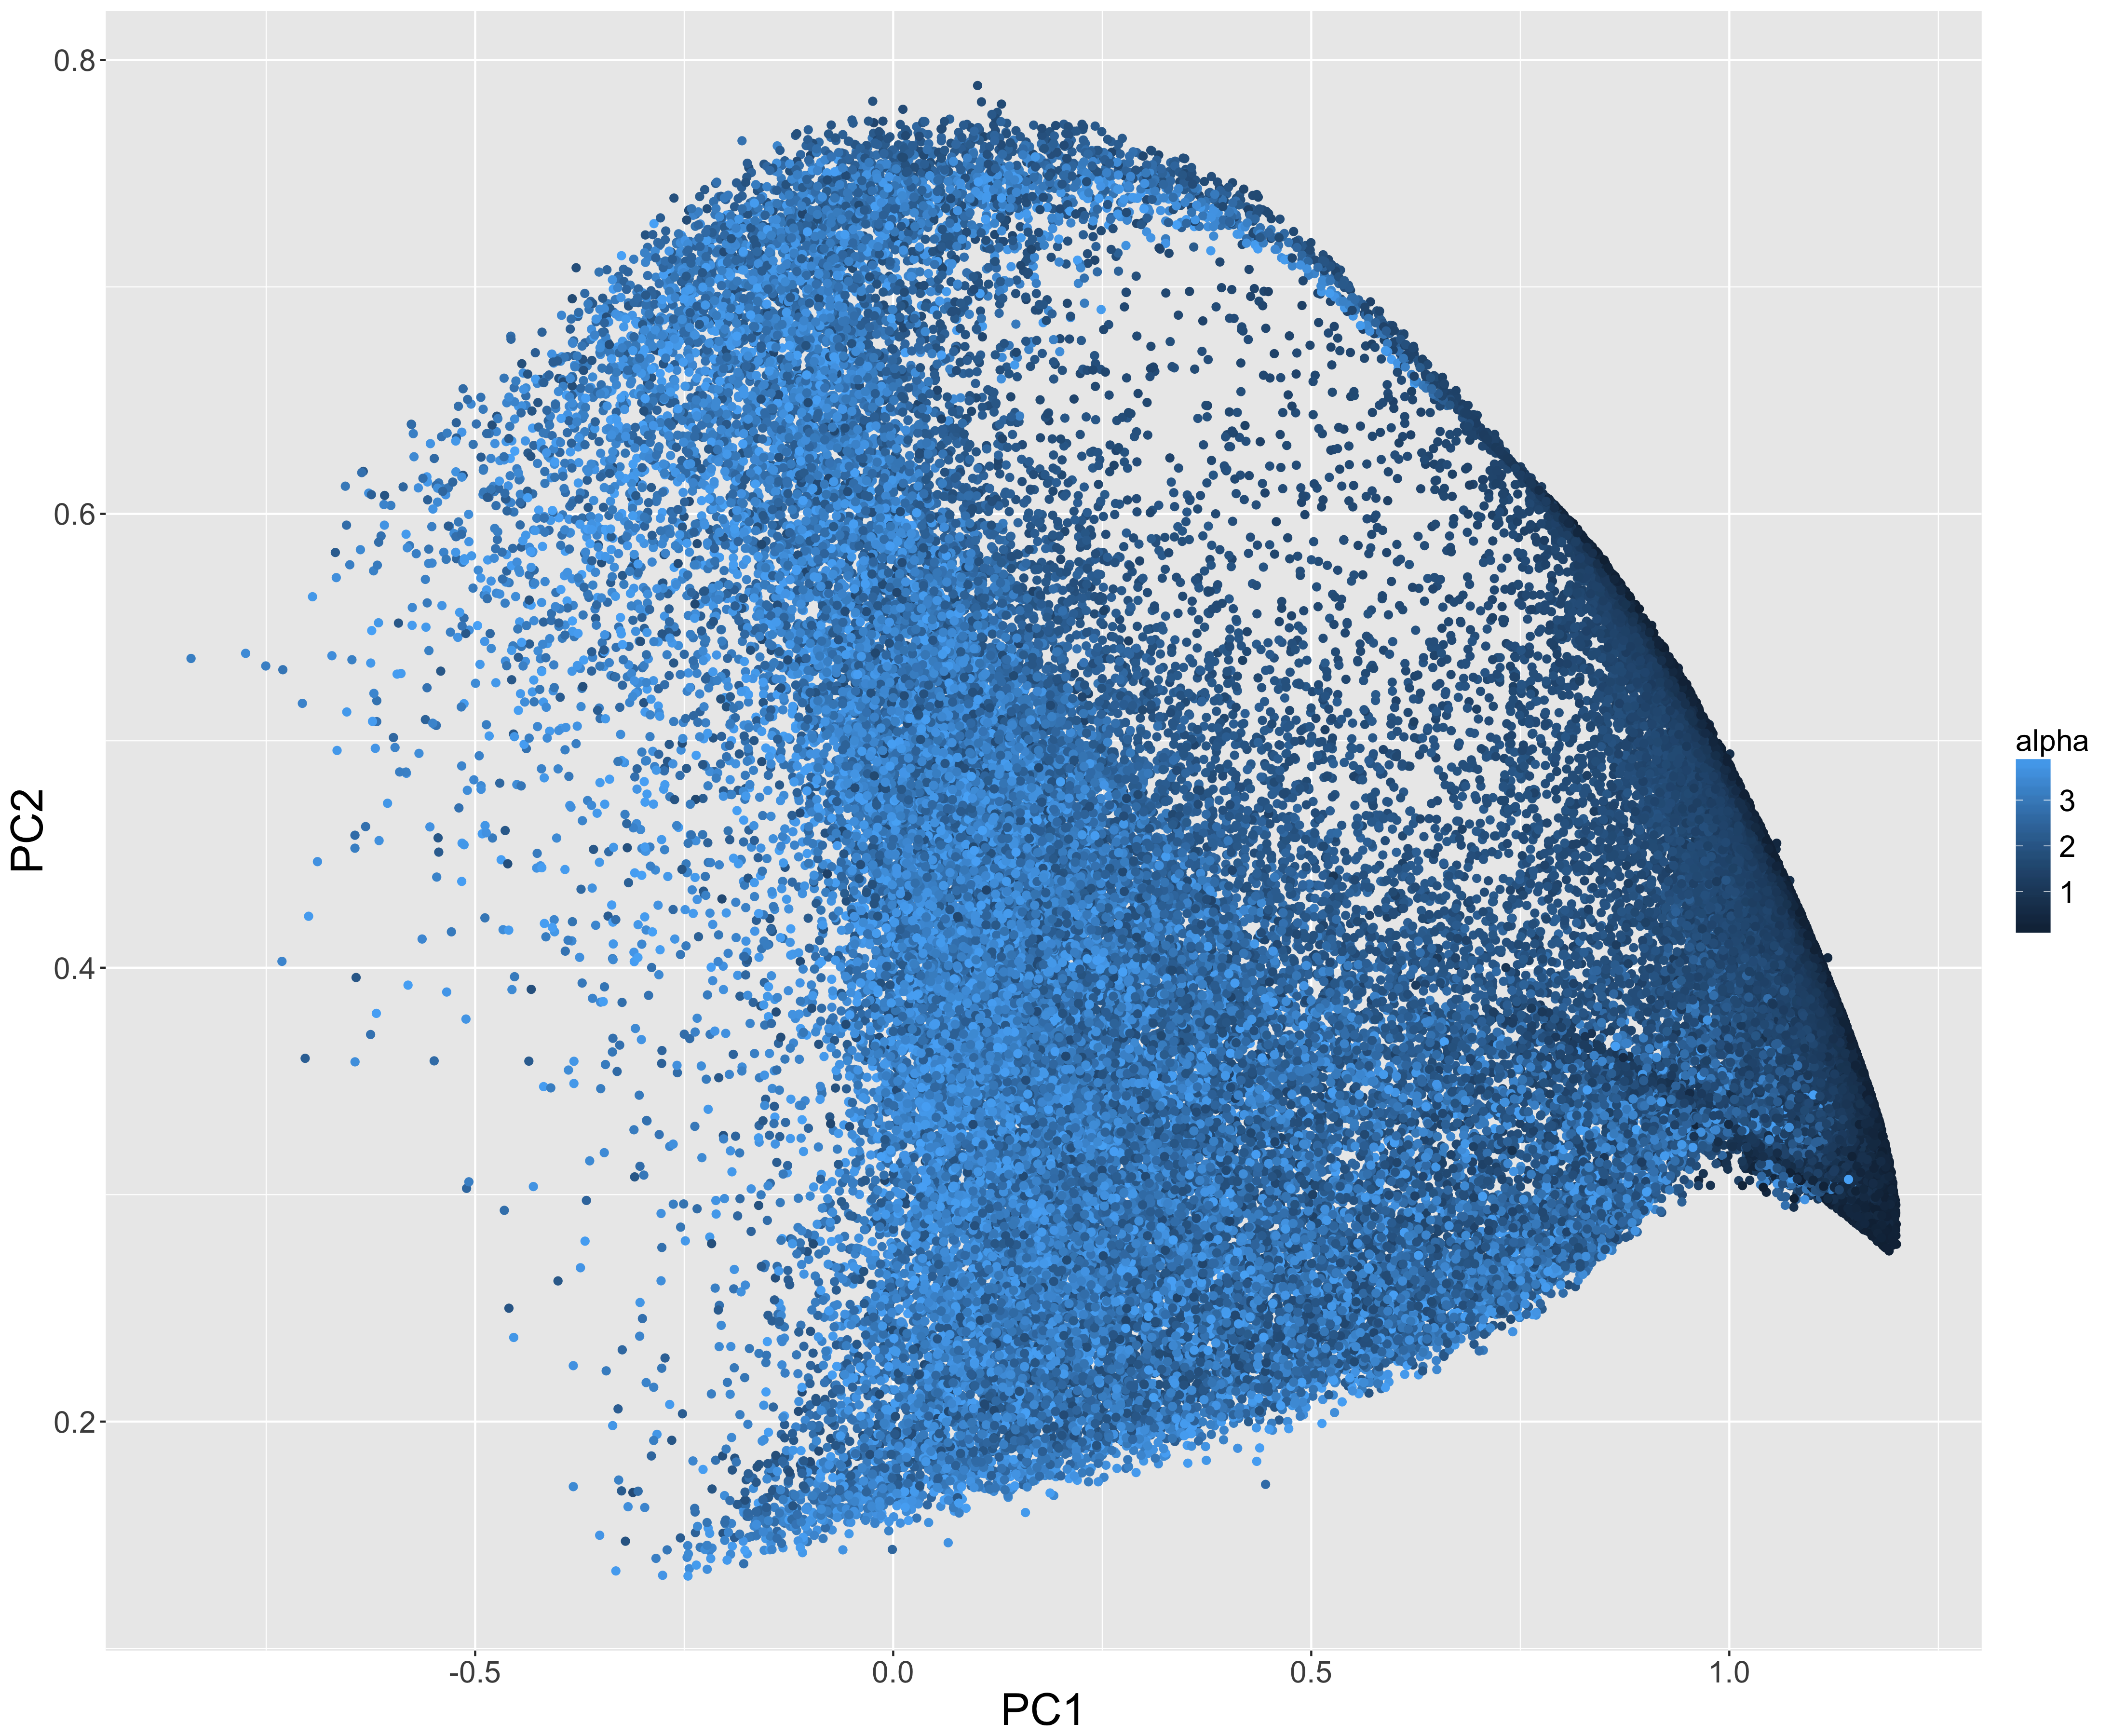
\includegraphics[width=0.5\textwidth]{figures/density_pc_colalpha}
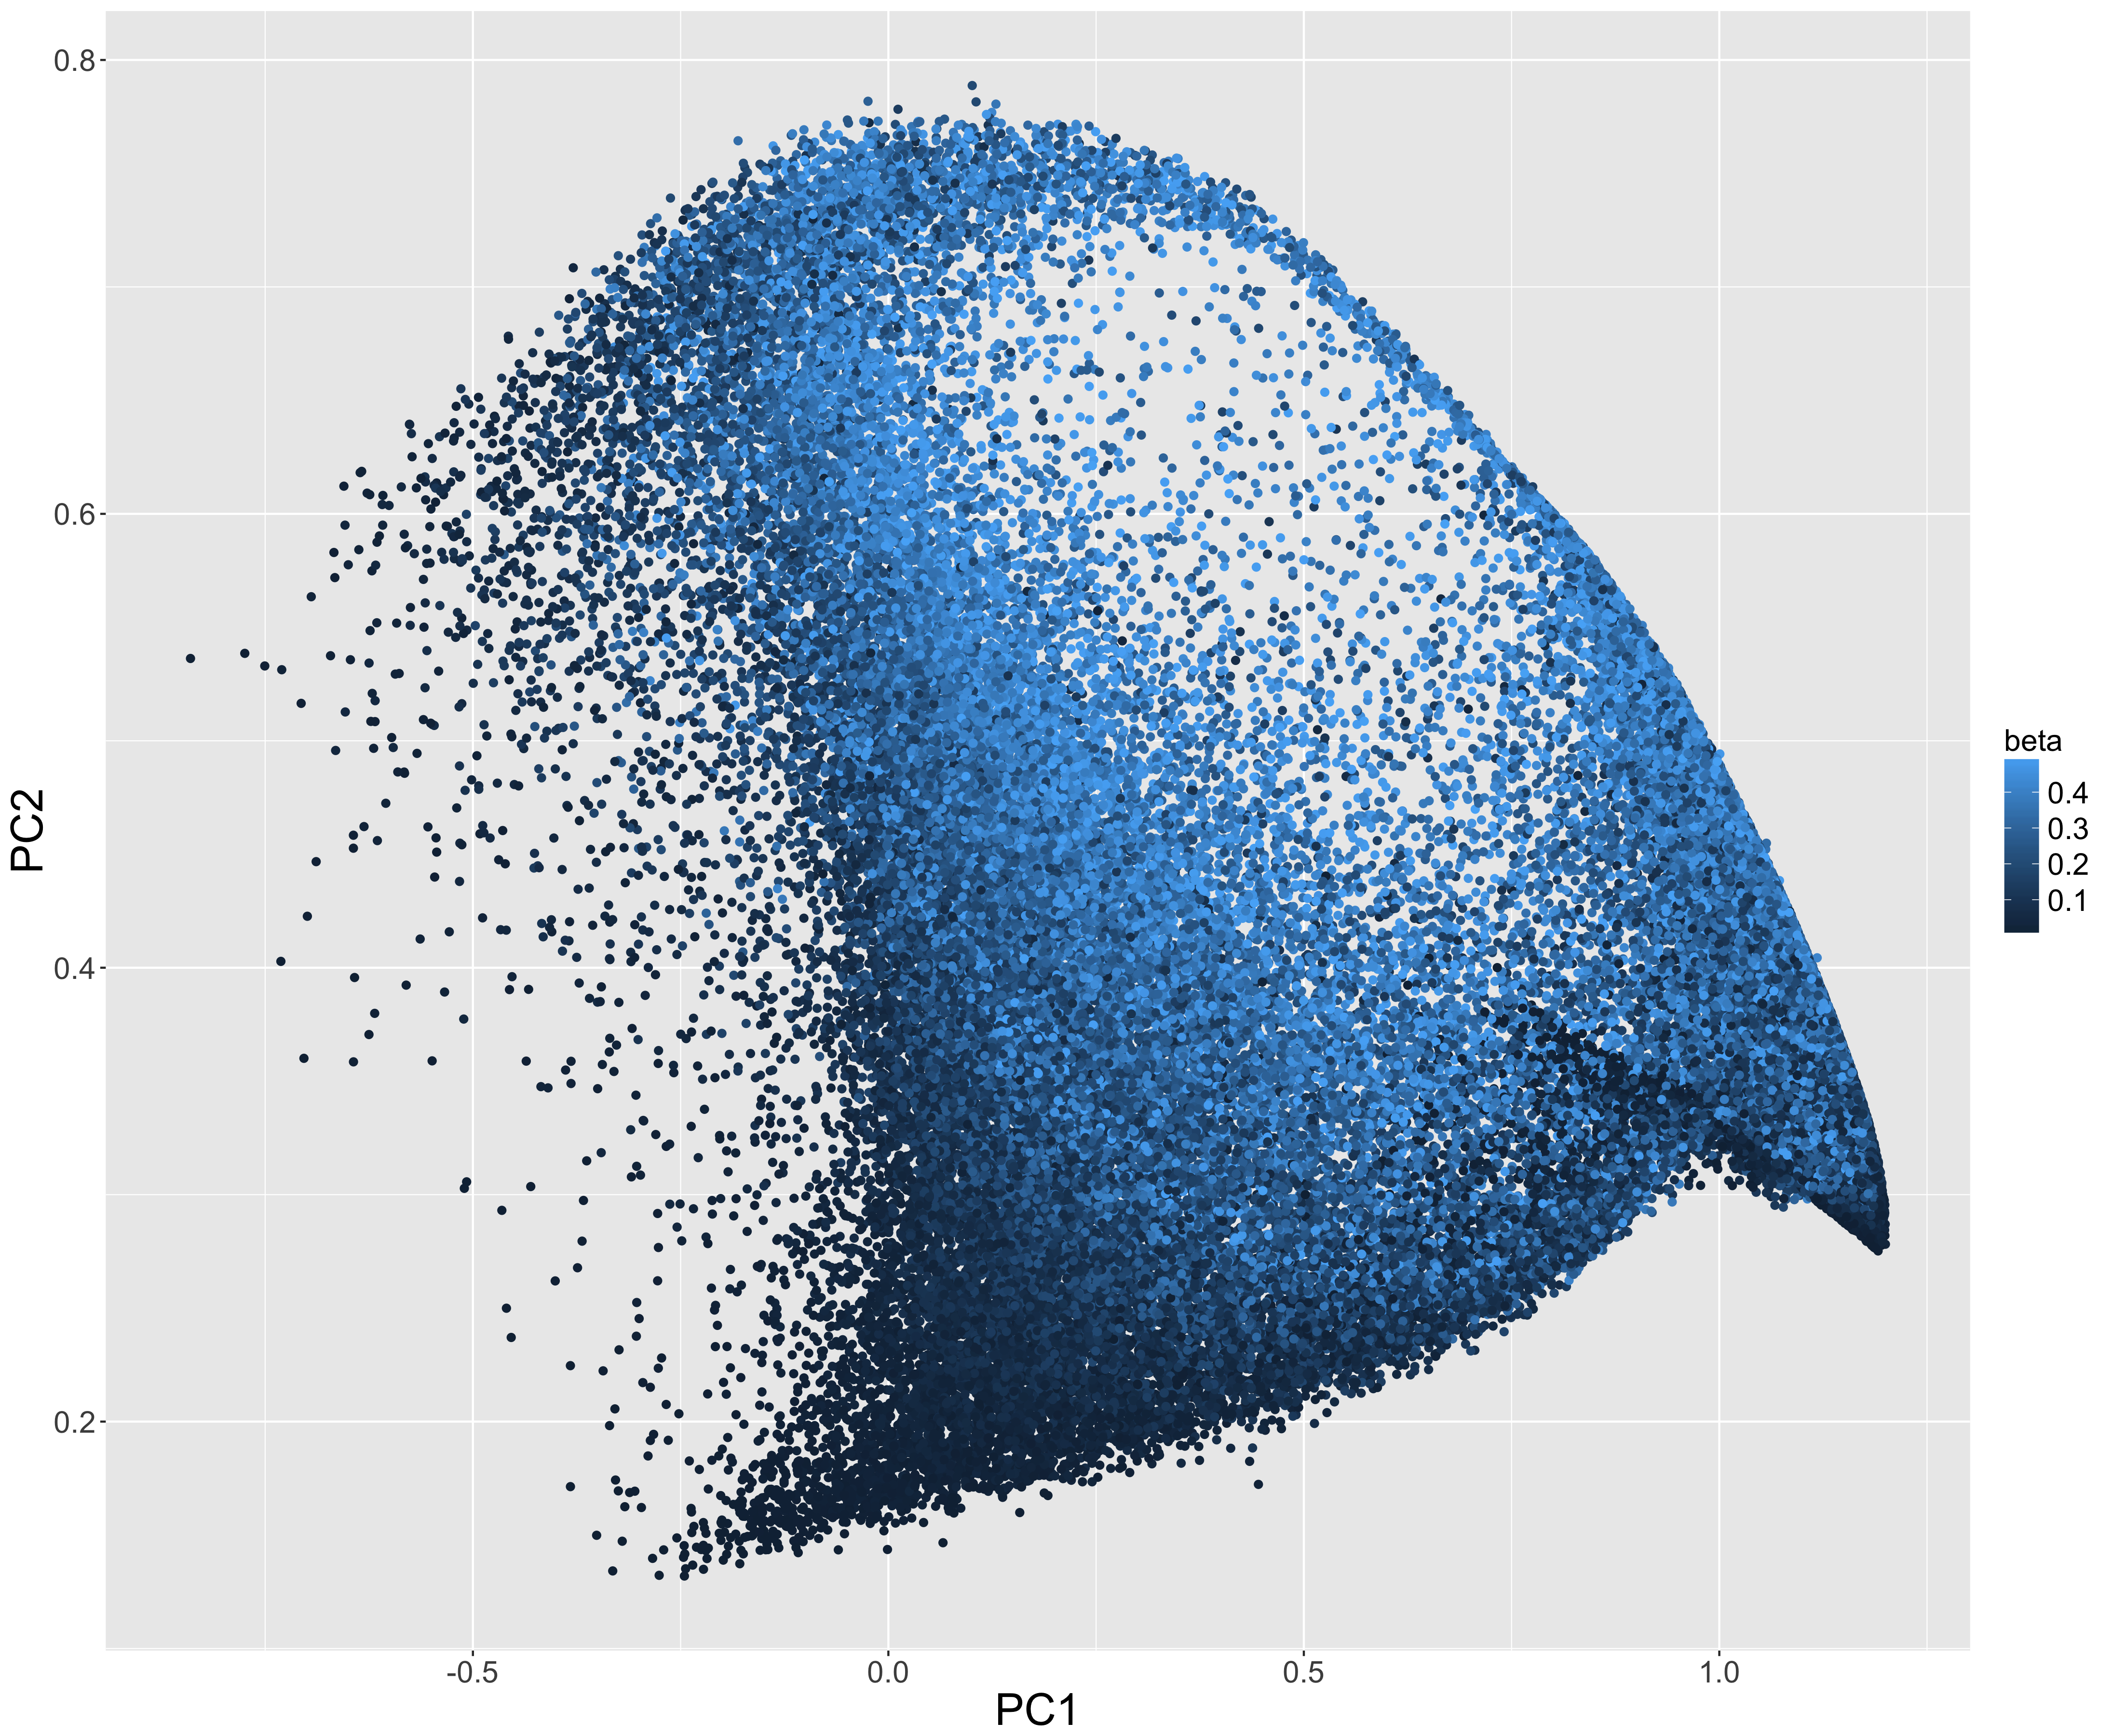
\includegraphics[width=0.5\textwidth]{figures/density_pc_colbeta}

}


\sframe{Empirical indicators computation}{

$\rightarrow$ Eurostat population density raster (100m, simplified at 500m resolution)

\medskip

$\rightarrow$ Overlapping (10km offset) squares of 50km side : equivalent to smoothing, removes window shape effect. Not very sensitive to window size (tested with 30km and 100km)

\medskip

$\rightarrow$ Indicators computed using Fast Fourier Transform Convolution

\medskip

$\rightarrow$ Classification using repeated k-means ; number of clusters taken at transition in clustering coefficient.

}

\sframe{Model calibration: all indicators}{

\centering
\includegraphics[width=0.65\textwidth]{figures/density_scatter}

}




%%%%%%%%%%%%%%%%%
%\section*{Co-evolution Morphogenesis}




\sframe{Defining co-evolution}{


\justify

No clear definition of co-evolution in the literature : \cite{bretagnolle:tel-00459720} distinguishes ``reciprocal adaptation'' where a sense of causality can clearly be identified, from co-evolutive regimes 


\bigskip
\bigskip

Identification of multiple causality regimes in a simple strongly coupled growth model $\rightarrow$ to be put in perspective with a theoretical definition of co-evolution based on the conjunction of Morphogenesis and the Evolutive Urban Theory, given in~\cite{raimbault2018caracterisation}

}


\sframe{Modeling Co-evolution}{

\justify

\cite{baptistemodeling} system dynamics with evolving capacities
 
\cite{wu2017city} population diffusion and network growth

\cite{blumenfeld2010network} and \cite{schmitt2014modelisation}: random potential breakdown for network growth.

\cite{barthelemy2009co} geometrical network growth model making network topology co-evolve with vertex density

}


\sframe{Empirical Data : network indicators}{

\centering

\includegraphics[width=0.53\textwidth]{figures/coevol_FR_indics_network_selected_2_discrquantiles}

}

\sframe{Empirical Data : correlations}{

\centering
\includegraphics[width=0.7\textwidth]{figures/coevol_FR_corr_PCA_rhoasize12}

}



\sframe{Network Indicators}{

Network Topology measured by:

\begin{itemize}
	\item Betweenness and Closeness centralities: average and hierarchy
	\item Accessibility (weighted closeness)
	\item Efficiency (network pace relative to euclidian distance)
	\item Mean path length, diameter
\end{itemize}

}




\sframe{Model specification}{

\footnotesize

Patch utility given by $U_i \textrm{ = } \sum_k w_k \cdot \tilde{x}_k$ with $\tilde{x}_k$ normalized local variables among population, betweenness and closeness centrality, distance to roads, accessibility ; aggregation done with probability $\left(U_i/\sum_k U_k\right)^\alpha$ ; diffusion among neighbors $n_d$ times with strength $\beta$

\medskip

\textbf{Network Generation:}

Adding a fixed number $n_N$ of new nodes: for patches such that $d_r < d_0$, probability to receive a node is

%% note : not a proba for the last ? no pb as soon as in 0,1, realized anyway.
\[
p \textrm{ = } P/P_{max} \cdot \left(d_M - d\right)/d_M \cdot \exp\left(-\left(\left(d_r - d_0\right)/\sigma_r\right)^2\right)
\]

Nodes connected the shortest way to existing network.

\medskip

\textbf{General model parameters :}

\begin{itemize}
	\item Patch utility weights $w_k$
	\item General network generation parameters: growth time steps $t_N$, maximal additional links
\end{itemize}

}



\sframe{Deterministic breakdown Network generation}{

\begin{enumerate}
\item Gravity potential given by
\[
V_{ij}\left(d\right) \textrm{ = } \left[ \left(1 - k_h\right) \textrm{ + } k_h \cdot \left( \frac{P_i P_j}{P^2} \right)^{\gamma} \right]\cdot \exp{\left( -\frac{d}{r_g \left(1 + d/d_0 \right)} \right)}
\]

\item $k\cdot N_L$ links are selected with lowest $V_{ij}(d_N)/V_{ij}(d_{ij})$, among which $N_L$ links with highest (lest costly) are realized
\item Network is planarized
\end{enumerate}
}


\sframe{Biological Network generation}{

Adding new links with biological heuristic:

\begin{enumerate}
	\item Create network of potential new links, with existing network and randomly sampled diagonal lattice
	\item Iterate for $k$ increasing ($k\in \{ 1,2,4 \}$ in practice) :
	\begin{itemize}
		\item Using population distribution, iterate $k\cdot n_b$ times the slime mould model to compute new link capacities
		\item Delete links with capacity under $\theta_d$
		\item Keep the largest connected component
	\end{itemize}
	\item Planarize and simplify final network
\end{enumerate}

}


\sframe{Model setup}{

\textbf{Synthetic setup: } rank-sized monocentric cities, simple connection with bord nodes to avoid bord effects 

\textbf{Real setup: } Population density raster at 500m resolution (European Union, from Eurostat)

\centering
\frame{\includegraphics[width=0.35\textwidth]{figures/coevol_example_synthsetup}}\hspace{0.1cm}
\frame{\includegraphics[width=0.35\textwidth]{figures/coevol_example-realsetup}}

\textbf{Stopping conditions: } fixed final time; fixed total population; fixed network size.

}


\sframe{Calibration Method}{


%% The model is calibrated at the first order (indicators of urban form and network measures) and at the second order (correlations) with Eurostat population grid coupled with street network from OpenStreetMap through the following workflow: indicators (Moran index, mean distance, hierarchy, entropy for morphology, mean path length, centralities, performance for network) are computed on real areas of width 50km for all Europe (what corresponds to the typical scale of processes the model includes); parameter space of the model is explored using grid computing (with OpenMole model exploration software), from simple synthetic initial configurations (few connected punctual settlements), computing indicators on final simulated configurations;  among candidate parameters for given contiguous (in space and indicator space) real areas on which correlations can be computed, the one with the closest correlation matrix computed on repetitions is chosen.



\begin{itemize}
	\item Brute force exploration of a LHS sampling, 10 repetitions of the model for each parameter point.
	\item For each simulated point, closest in indicator space (euclidian distance for normalized indicators) among real points are selected.
	\item Among these, point with lowest distance to correlation matrix are taken.
\end{itemize}


}

\sframe{Calibration: optimal points}{

\centering

\includegraphics[width=0.45\textwidth]{figures/coevol_dists_pareto_i1}
\includegraphics[width=0.45\textwidth]{figures/coevol_dists_pareto_i10}

\footnotesize\textit{Pareto plots of distance to indicators and distance to correlation matrices, for a given simulated configuration and all real points.}

}



\sframe{Causality regimes: clustering}{

\centering

\includegraphics[width=0.48\textwidth]{figures/coevol_clustcoef}
\includegraphics[width=0.48\textwidth]{figures/coevol_diffclustcoef}

\medskip

\footnotesize\textit{Clustering coefficient (left) and its derivative (right) as a function of number of clusters}

}




%%%%%%%%%%%%%%%%%%%%%
\begin{frame}[allowframebreaks]
\frametitle{References}
\bibliographystyle{apalike}
\bibliography{biblio}
\end{frame}
%%%%%%%%%%%%%%%%%%%%%%%%%%%%





\end{document}






